\documentclass{scutthesis}

% 开始使用该模板请修改以下文件
%%
% 课程报告相关信息
%%

% 标题
\covertitlefirst{代码覆盖率及路径分析检测工具}
\covertitlesecond{课程大作业报告}

\etitlefirst{Code Coverage and Path Analysis Tool}
\etitlesecond{Course Project Report}

% 中文标题
\ctitle{代码覆盖率及路径分析检测工具}
\etitle{Code Coverage and Path Analysis Tool}

% 作者详细信息
\author{许同学}
\cauthor{许\ 同\ 学}
\eauthor{Xu}
\studentid{2023000000}
\cschool{计算机学院}

\cmajor{软件工程}
\emajor{Software Engineering}

\phonenum{13800138000}
\mailbox{student@university.edu}

% 指导老师
\cmentor{张老师\ (副教授)}
\ementor{Prof. Zhang}
     % 在这里填写论文相关信息

\begin{document}
% 论文前置部分
\frontmatter
\pagenumbering{Roman}
\makeUndergraduateCover    % 生成封面

\maketableofcontents        % 生成目录

% 论文主体部分
\mainmatter

%%
% 第一章：项目背景与实验目标
%%

\chapter{项目背景与实验目标}
\label{chap:background}

\section{PageIndex项目概述}

PageIndex是一个基于LangChain框架的智能文档问答系统，其核心功能是对索引文档进行语义搜索并生成基于文档内容的回答。该系统采用PostgreSQL作为后端存储，支持对大量文档进行高效管理和检索。从技术架构上看， PageIndex系统主要包含三个核心模块：文档索引模块负责将PDF、Markdown等格式的文档解析为结构化的树形数据并存储到数据库中； 文档搜索模块接收用户的自然语言查询,首先通过大语言模型从文档目录中选择最相关的文档，然后在这些文档的结构树中搜索相关节点，最后将搜索结果组装成上下文并生成最终答案; LangChain集成模块将整个搜索流程封装为LangChain工具，使其可以方便地集成到AI Agent应用中。

PageIndex项目的代码结构清晰地体现了这一设计理念。核心文件\texttt{search.py}（约400行）实现了完整的搜索流程， 包括数据模型定义、文档选择、并发搜索、上下文构建等关键功能。该文件定义了\texttt{CatalogEntry}、\texttt{RelevantNode}、\texttt{DocumentSearchResult}、\texttt{PageIndexSearchResult}等数据类来封装中间结果， 并通过\texttt{run\_tree\_search}函数协调整个搜索流程。另一个核心文件\texttt{page\_index.py}（约2000行）实现了文档解析和索引的底层逻辑， 包含大量的异步处理、并发控制和条件分支， 这些复杂的控制流结构使其成为代码覆盖率分析的理想测试对象。

从程序结构角度分析, PageIndex项目代码包含了丰富的控制流特征。在顺序结构方面, 代码包含大量的数据处理流程, 如JSON解析、数据转换、结果格式化等。在选择结构方面, 代码中广泛使用了if/elif/else语句进行条件判断, 包括参数验证（如检查\texttt{doc\_top\_k}是否大于0）、类型检查（如判断payload是否为dict或list）、状态判断（如判断搜索是否成功）等。在循环结构方面, 代码使用了for循环遍历文档列表和节点树, 使用while循环进行栈式遍历, 并通过asyncio实现并发控制。此外, 代码还包含异常处理结构, 对数据库操作、API调用等可能失败的操作进行异常捕获。这些丰富的控制流结构为执行路径追踪和覆盖率分析提供了充分的测试场景。

\section{实验目标与要求}

本次课程作业的核心目标是设计并实现一个能够记录Python程序执行路径和覆盖率的工具。根据作业要求, 该工具需要满足以下功能: 能够记录Python程序的执行路径和覆盖率; 能够分析基本程序常见结构流, 包括选择、顺序与循环; 能够记录程序运行时的执行路径; 能够生成描述程序运行执行分支的报告。同时, 代码需要有必要的注释和说明使用文档, 程序结构需要清晰且具有一定的可扩展性。

为了实现这些目标, 我们设计了PathTracer工具, 它是一个专门用于追踪Python程序执行路径和计算代码覆盖率的工具。与现有的coverage.py等工具相比, PathTracer的独特之处在于它同时结合了静态分析和动态追踪两种技术: 通过AST静态分析识别源代码中的所有控制流分支点, 通过运行时追踪记录实际执行的代码路径, 然后通过对比两者来计算覆盖率。此外, PathTracer还具备函数调用树追踪功能, 能够记录函数调用的参数和返回值, 这对于理解程序的执行行为具有重要价值。

\section{技术背景}

在实现PathTracer工具之前, 我们需要了解几个关键技术。首先是Python的\texttt{sys.settrace}机制, 这是Python解释器提供的运行时追踪接口。当通过\texttt{sys.settrace(trace\_callback)}注册一个回调函数后, Python解释器会在程序执行过程中每当发生特定事件时调用该回调。这些事件包括: 'call'事件在函数被调用时触发; 'line'事件在即将执行新的一行代码时触发; 'return'事件在函数返回时触发; 'exception'事件在发生异常时触发。通过处理这些事件, 我们可以精确记录程序的执行轨迹。需要注意的是, \texttt{sys.settrace}会带来显著的性能开销, 程序执行速度可能降低10到100倍, 因此该技术更适合教学演示、调试分析等场景, 而不适合在生产环境中常驻使用。

第二个关键技术是Python的\texttt{ast}模块, 它可以将源代码解析为抽象语法树。AST是源代码的树形表示, 其中每个节点代表代码中的一个结构。通过遍历AST, 我们可以识别源代码中的所有控制流结构, 包括\texttt{ast.If}（if条件语句）、\texttt{ast.For}（for循环）、\texttt{ast.While}（while循环）、\texttt{ast.ExceptHandler}（异常处理器）等。这种静态分析方法使我们能够在不执行程序的情况下获取代码的完整结构信息, 这是计算代码覆盖率的基础——我们需要知道代码中有哪些分支点, 然后才能判断哪些分支在运行时被执行了。

代码覆盖率是软件测试领域的重要概念, 用于衡量测试用例对被测代码的覆盖程度。常见的覆盖率类型包括: 语句覆盖测量被执行的代码语句比例; 分支覆盖测量控制流分支的执行比例, 如if语句的true/false两个分支是否都被执行; 路径覆盖测量程序执行路径的覆盖比例。本实验主要关注分支覆盖, 即识别程序中的控制流分支点, 并统计在运行时被触发的分支数量。覆盖率公式为: 覆盖率 = (已执行分支数 / 总分支数) × 100\%。需要注意的是, 高覆盖率本身不是目的, 重要的是覆盖的有效性——如果未覆盖的分支主要是防御性代码（如空值检查、异常处理）或互斥逻辑（不可能同时执行的分支）, 那么即使覆盖率不是100\%也是可以接受的。
 % 第一章：实验目的和背景
\newclearpage
%%
% 第二章：系统设计与实现
%%

\chapter{系统设计与实现}
\label{chap:design}

\section{系统架构}

PathTracer系统采用模块化设计，由以下核心组件构成：

\begin{figure}[htbp]
    \centering
    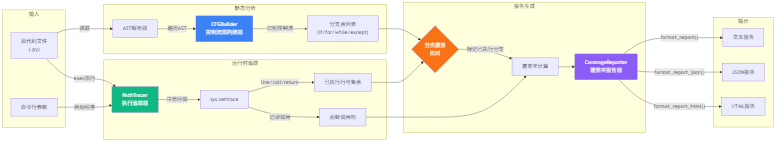
\includegraphics[width=0.95\textwidth]{figures/pathtracer-architecture.png}
    \caption{PathTracer系统架构图}
    \label{fig:architecture}
\end{figure}

\subsection{模块划分}

系统主要包含以下模块：

\begin{table}[htbp]
    \centering
    \caption{模块职责划分}
    \label{tab:modules}
    \begin{tabular}{llp{6cm}}
        \toprule
        \textbf{模块} & \textbf{文件} & \textbf{核心职责} \\
        \midrule
        数据模型 & models.py & 定义分支类型枚举、代码分支、函数调用、执行路径、覆盖率报告等数据结构 \\
        运行时追踪 & tracer.py & 使用\texttt{sys.settrace}追踪程序执行，记录行号和函数调用 \\
        控制流分析 & cfg\_builder.py & 使用AST静态分析识别源代码中的所有分支点 \\
        报告生成 & reporter.py & 对比静态分支与执行路径，计算覆盖率，生成多格式报告 \\
        命令行接口 & cli.py & 解析命令行参数，协调各模块工作流程 \\
        \bottomrule
    \end{tabular}
\end{table}

\section{核心数据模型}

\subsection{分支类型枚举}

定义了程序中可能出现的控制流分支类型：

\begin{lstlisting}[language=Python, caption=分支类型枚举定义]
class BranchType(Enum):
    """控制流分支类型枚举"""
    SEQUENTIAL = "sequential"  # 顺序执行
    IF = "if"                  # if条件语句
    ELSE = "else"              # else分支
    ELIF = "elif"              # elif分支
    FOR = "for"                # for循环
    WHILE = "while"            # while循环
    TRY = "try"                # try异常捕获块
    EXCEPT = "except"          # except异常处理块
\end{lstlisting}

\subsection{代码分支数据类}

\texttt{CodeBranch}表示源代码中的一个分支点：

\begin{lstlisting}[language=Python, caption=CodeBranch数据类]
@dataclass
class CodeBranch:
    """表示代码中的一个分支点"""
    file_path: str           # 源文件路径
    line_no: int             # 分支起始行号
    branch_type: BranchType  # 分支类型
    end_line: int = 0        # 分支结束行号
    is_executed: bool = False # 运行时是否被执行
\end{lstlisting}

\subsection{函数调用记录类}

\texttt{FunctionCall}记录函数调用信息，支持嵌套调用树：

\begin{lstlisting}[language=Python, caption=FunctionCall数据类]
@dataclass
class FunctionCall:
    """记录函数调用信息"""
    function_name: str              # 函数名
    file_path: str                  # 所在文件
    line_no: int                    # 调用行号
    call_depth: int                 # 调用深度（0为顶层）
    arguments: Dict[str, str]       # 参数名到值的映射
    return_value: Optional[str]     # 返回值（repr后的字符串）
    children: List['FunctionCall']  # 子调用列表
\end{lstlisting}

\subsection{覆盖率报告类}

\texttt{CoverageReport}汇总分析结果：

\begin{lstlisting}[language=Python, caption=CoverageReport数据类]
@dataclass
class CoverageReport:
    """覆盖率分析报告"""
    total_branches: int = 0           # 总分支数
    executed_branches: int = 0        # 已执行分支数
    branches_by_type: Dict[BranchType, int]  # 按类型统计
    coverage_percentage: float = 0.0  # 覆盖率百分比
    file_reports: Dict[str, ExecutionPath]   # 各文件详细报告
\end{lstlisting}

\section{运行时追踪器实现}

\subsection{sys.settrace机制原理}

Python的\texttt{sys.settrace}函数允许注册一个全局追踪回调。当程序执行时，解释器会在每个"事件"发生时调用该回调：

\begin{table}[htbp]
    \centering
    \caption{追踪事件类型}
    \label{tab:events}
    \begin{tabular}{lp{8cm}}
        \toprule
        \textbf{事件} & \textbf{触发时机} \\
        \midrule
        'call' & 函数被调用时（进入函数体前） \\
        'line' & 即将执行新的一行代码时 \\
        'return' & 函数即将返回时（arg为返回值） \\
        'exception' & 发生异常时（arg为异常元组） \\
        \bottomrule
    \end{tabular}
\end{table}

\subsection{追踪回调函数核心实现}

\begin{lstlisting}[language=Python, caption=追踪回调函数实现]
def _trace_callback(self, frame, event: str, arg):
    """内部追踪回调函数

    Args:
        frame: 当前栈帧对象，包含代码对象、局部变量等
        event: 事件类型 ('call', 'line', 'return', 'exception')
        arg: 事件相关参数 (return时为返回值，exception时为异常信息)

    Returns:
        返回自身以继续追踪，或None停止追踪
    """
    if not self._target_file:
        return None

    code = frame.f_code
    # 只追踪目标文件
    if not code.co_filename.endswith(self._target_file):
        return self._trace_callback

    if event == 'line':
        # 记录执行的行号
        line_no = frame.f_lineno
        self.execution_paths[self._target_file] \
            .executed_lines.add(line_no)

    elif event == 'call':
        # 提取函数名和参数
        func_name = code.co_name
        args = self._extract_arguments(frame, code)
        # 构建函数调用对象
        call_depth = len(self._call_stack)
        func_call = FunctionCall(
            function_name=func_name,
            file_path=code.co_filename,
            line_no=frame.f_lineno,
            call_depth=call_depth,
            arguments=args
        )
        # 添加到调用树
        if self._call_stack:
            self._call_stack[-1].children.append(func_call)
        else:
            self.function_calls.append(func_call)
        self._call_stack.append(func_call)

    elif event == 'return':
        # 弹出调用栈，记录返回值
        if self._call_stack:
            func_call = self._call_stack.pop()
            if arg is not None:
                func_call.return_value = repr(arg)

    return self._trace_callback
\end{lstlisting}

\subsection{参数提取实现}

\begin{lstlisting}[language=Python, caption=函数参数提取]
def _extract_arguments(self, frame, code) -> Dict[str, str]:
    """从栈帧中提取函数参数

    利用code对象获取参数名列表，从frame.f_locals获取参数值
    """
    args = {}
    try:
        arg_count = code.co_argcount
        arg_names = code.co_varnames[:arg_count]
        for arg_name in arg_names:
            if arg_name in frame.f_locals:
                try:
                    args[arg_name] = repr(frame.f_locals[arg_name])
                except Exception:
                    args[arg_name] = '<unable to repr>'
    except Exception:
        pass
    return args
\end{lstlisting}

\subsection{上下文管理器接口}

使用Python的上下文管理器协议简化追踪的启动和停止：

\begin{lstlisting}[language=Python, caption=上下文管理器实现]
def __enter__(self):
    """进入上下文：保存原追踪函数，启动追踪"""
    self._original_trace = sys.gettrace()
    sys.settrace(self._trace_callback)
    return self

def __exit__(self, exc_type, exc_val, exc_tb):
    """退出上下文：恢复原追踪函数"""
    sys.settrace(self._original_trace)
    return False  # 不抑制异常
\end{lstlisting}

使用示例：
\begin{lstlisting}[language=Python]
tracer = PathTracer().trace_file("target.py")
with tracer:
    # 在此执行目标代码
    result = target_function()
# 退出with块后自动停止追踪
\end{lstlisting}

\section{控制流图构建器}

\subsection{AST遍历原理}

Python的\texttt{ast}模块可以将源代码解析为抽象语法树。通过遍历AST，可以识别所有控制流节点：

\begin{lstlisting}[language=Python, caption=AST遍历构建CFG]
def build_from_file(self, file_path: str) -> List[CodeBranch]:
    """从Python文件构建控制流图

    Args:
        file_path: Python源文件路径

    Returns:
        识别到的所有分支点列表
    """
    with open(file_path, 'r', encoding='utf-8') as f:
        source = f.read()

    # 解析源代码为AST
    tree = ast.parse(source, filename=file_path)
    self.branches = []

    # 遍历AST，提取控制流节点
    for node in ast.walk(tree):
        branch = self._extract_branch(file_path, node)
        if branch:
            self.branches.append(branch)

    return self.branches
\end{lstlisting}

\subsection{分支节点识别}

\begin{lstlisting}[language=Python, caption=分支节点识别逻辑]
def _extract_branch(self, file_path: str, node: ast.AST):
    """从AST节点提取分支信息

    识别if/for/while/except等控制流结构
    """
    # if条件语句
    if isinstance(node, ast.If):
        return CodeBranch(
            file_path=file_path,
            line_no=node.lineno,
            branch_type=BranchType.IF,
            end_line=self._get_end_line(node)
        )

    # for循环
    elif isinstance(node, ast.For):
        return CodeBranch(
            file_path=file_path,
            line_no=node.lineno,
            branch_type=BranchType.FOR,
            end_line=self._get_end_line(node)
        )

    # while循环
    elif isinstance(node, ast.While):
        return CodeBranch(
            file_path=file_path,
            line_no=node.lineno,
            branch_type=BranchType.WHILE,
            end_line=self._get_end_line(node)
        )

    # except异常处理器
    elif isinstance(node, ast.ExceptHandler):
        return CodeBranch(
            file_path=file_path,
            line_no=node.lineno,
            branch_type=BranchType.EXCEPT,
            end_line=self._get_end_line(node)
        )

    return None
\end{lstlisting}

\subsection{结束行号计算}

\begin{lstlisting}[language=Python, caption=结束行号计算]
def _get_end_line(self, node: ast.AST) -> int:
    """获取代码块的结束行号

    优先使用Python 3.8+的end_lineno属性，
    否则递归计算body中最大的行号
    """
    # Python 3.8+ 提供end_lineno属性
    if hasattr(node, 'end_lineno') and node.end_lineno is not None:
        return node.end_lineno

    # 递归计算body中的最大行号
    if hasattr(node, 'body') and node.body:
        return max(self._get_end_line(n) for n in node.body)

    return getattr(node, 'lineno', 0)
\end{lstlisting}

\section{报告生成器}

\subsection{覆盖率计算核心逻辑}

\begin{lstlisting}[language=Python, caption=覆盖率计算实现]
def analyze(self, file_path: str, tracer: PathTracer) -> CoverageReport:
    """分析覆盖率

    Args:
        file_path: 要分析的文件路径
        tracer: 已执行追踪的PathTracer实例

    Returns:
        CoverageReport: 覆盖率报告对象
    """
    # 1. 静态分析：获取所有分支点
    all_branches = self.cfg_builder.build_from_file(file_path)

    # 2. 动态追踪：获取已执行行号
    executed_lines = tracer.get_executed_lines(file_path)

    # 3. 标记已执行的分支
    for branch in all_branches:
        if branch.line_no in executed_lines:
            branch.is_executed = True

    # 4. 计算统计指标
    total = len(all_branches)
    executed = sum(1 for b in all_branches if b.is_executed)

    # 5. 按类型统计
    by_type: Dict[BranchType, int] = {}
    for branch_type in BranchType:
        type_branches = [b for b in all_branches
                        if b.branch_type == branch_type]
        by_type[branch_type] = len(type_branches)

    # 6. 构建报告对象
    return CoverageReport(
        total_branches=total,
        executed_branches=executed,
        branches_by_type=by_type,
        coverage_percentage=(executed / total * 100) if total > 0 else 0.0,
        file_reports={file_path: ExecutionPath(...)}
    )
\end{lstlisting}

\subsection{覆盖率计算公式}

覆盖率计算公式：

\begin{equation}
    \label{eq:coverage}
    \text{Coverage} = \frac{N_{executed}}{N_{total}} \times 100\%
\end{equation}

其中：
\begin{itemize}
    \item $N_{total}$：静态分析识别的总分支数
    \item $N_{executed}$：运行时实际执行的分支数
\end{itemize}

\subsection{多格式报告输出}

\begin{table}[htbp]
    \centering
    \caption{报告输出格式}
    \label{tab:format}
    \begin{tabular}{llp{5cm}}
        \toprule
        \textbf{格式} & \textbf{方法} & \textbf{特点} \\
        \midrule
        文本 & format\_report() & 纯文本，适合控制台输出 \\
        JSON & format\_report\_json() & 结构化数据，便于程序处理 \\
        HTML & format\_report\_html() & 带语法高亮，适合可视化查看 \\
        \bottomrule
    \end{tabular}
\end{table}

\section{HTML报告生成}

\subsection{HTML报告结构}

HTML报告包含以下部分：

\begin{enumerate}
    \item \textbf{摘要卡片}：覆盖率百分比、总分支数、已执行分支数
    \item \textbf{分支类型统计}：按if/for/while/except分类的统计
    \item \textbf{源代码展示}：带行号和执行状态高亮的代码
    \item \textbf{函数调用树}：嵌套展示函数调用关系
\end{enumerate}

\subsection{执行状态视觉区分}

\begin{table}[htbp]
    \centering
    \caption{代码行状态样式}
    \label{tab:styles}
    \begin{tabular}{lll}
        \toprule
        \textbf{状态} & \textbf{背景色} & \textbf{边框} \\
        \midrule
        已执行 & 绿色半透明 (\texttt{rgba(40,167,69,0.15)}) & 绿色左边框 \\
        未执行 & 红色半透明 (\texttt{rgba(220,53,69,0.15)}) & 红色左边框 \\
        \bottomrule
    \end{tabular}
\end{table}

\section{本章小结}

本章详细介绍了PathTracer系统的设计与实现：

\begin{enumerate}
    \item \textbf{数据模型}：使用Python dataclass定义分支类型、代码分支、函数调用、覆盖率报告等核心数据结构
    \item \textbf{运行时追踪}：基于\texttt{sys.settrace}实现，支持line/call/return事件追踪
    \item \textbf{静态分析}：基于AST遍历识别if/for/while/except控制流结构
    \item \textbf{报告生成}：支持文本/JSON/HTML三种输出格式
\end{enumerate}

整个系统仅依赖Python标准库，无需安装第三方依赖，具有良好的可移植性。
 % 第二章：系统设计与实现
\newclearpage
%%
% 第三章：实验过程与结果
%%

\chapter{实验过程与结果}
\label{chap:experiment}

\section{实验环境}

\begin{table}[htbp]
    \centering
    \caption{实验环境配置}
    \label{tab:env}
    \begin{tabular}{ll}
        \toprule
        \textbf{项目} & \textbf{配置} \\
        \midrule
        操作系统 & Windows 11 Pro \\
        Python版本 & 3.10+ \\
        依赖 & 无第三方依赖（使用标准库） \\
        开发工具 & VS Code / PyCharm \\
        \bottomrule
    \end{tabular}
\end{table}

\section{测试目标程序}

\subsection{程序简介}

本实验使用\texttt{agent\_pageindex.py}作为测试目标程序。该程序是一个基于LangChain的文档问答代理，具有以下特点：

\begin{itemize}
    \item 多层条件判断（参数验证、类型检查）
    \item 循环结构（消息处理、工具调用遍历）
    \item 函数调用（包含嵌套调用）
    \item 异常处理（API密钥检查）
\end{itemize}

\subsection{程序结构分析}

目标程序共130行代码，包含：

\begin{itemize}
    \item \texttt{\_extract\_text()}：文本提取辅助函数
    \item \texttt{\_print\_verbose\_stream()}：详细输出流处理函数
    \item \texttt{main()}：主函数，包含参数解析和Agent执行逻辑
\end{itemize}

\section{实验过程}

\subsection{运行测试}

使用PathTracer命令行工具对目标程序进行追踪：

\begin{lstlisting}[language=bash, caption=测试命令]
# 生成HTML格式报告
python -m pathtracer.cli -f html \
    -o coverage_report.html \
    agent_pageindex.py -- --query "test"

# 生成JSON格式报告
python -m pathtracer.cli -f json \
    -o coverage_report.json \
    agent_pageindex.py -- --query "test"
\end{lstlisting}

\subsection{测试用例设计}

为了验证工具功能，设计了以下测试用例：

\begin{table}[htbp]
    \centering
    \caption{测试用例}
    \label{tab:testcase}
    \begin{tabular}{lll}
        \toprule
        \textbf{编号} & \textbf{测试内容} & \textbf{参数} \\
        \midrule
        TC1 & 基本查询功能 & --query "test" \\
        TC2 & 详细输出模式 & --query "test" --verbose \\
        TC3 & 自定义参数 & --query "test" --doc-top-k 5 \\
        \bottomrule
    \end{tabular}
\end{table}

\section{实验结果}

\subsection{覆盖率统计}

执行TC1测试用例后的覆盖率统计结果：

\begin{table}[htbp]
    \centering
    \caption{覆盖率统计结果}
    \label{tab:coverage}
    \begin{tabular}{ll}
        \toprule
        \textbf{指标} & \textbf{数值} \\
        \midrule
        总分支数 & 22 \\
        已执行分支数 & 7 \\
        覆盖率 & 31.8\% \\
        \bottomrule
    \end{tabular}
\end{table}

\subsection{分支类型分布}

\begin{table}[htbp]
    \centering
    \caption{分支类型分布}
    \label{tab:branch-type}
    \begin{tabular}{lcc}
        \toprule
        \textbf{分支类型} & \textbf{总数} & \textbf{已执行} \\
        \midrule
        if语句 & 17 & 5 \\
        for循环 & 5 & 2 \\
        while循环 & 0 & 0 \\
        except块 & 0 & 0 \\
        \bottomrule
    \end{tabular}
\end{table}

\subsection{已执行分支详情}

\begin{table}[htbp]
    \centering
    \caption{已执行分支列表}
    \label{tab:executed}
    \begin{tabular}{cccl}
        \toprule
        \textbf{行号} & \textbf{分支类型} & \textbf{结束行} & \textbf{代码内容} \\
        \midrule
        25 & if & 26 & payload is None检查 \\
        27 & if & 28 & isinstance(payload, str)检查 \\
        88 & if & 89 & API密钥检查 \\
        116 & if & 118 & verbose模式检查 \\
        121 & if & 125 & result类型检查 \\
        123 & if & 125 & messages存在检查 \\
        129 & if & 130 & \_\_main\_\_入口检查 \\
        \bottomrule
    \end{tabular}
\end{table}

\subsection{函数调用树}

实验过程中记录的函数调用关系：

\begin{lstlisting}[caption=函数调用树]
main()
  load_dotenv()
  os.getenv("DEEPSEEK_API_KEY")
  init_chat_model()
  create_agent()
  agent.invoke()
  _extract_text()
  print()
\end{lstlisting}

\section{结果分析}

\subsection{覆盖率分析}

覆盖率为31.8\%，主要原因：

\begin{enumerate}
    \item \textbf{verbose模式未触发}：\texttt{\_print\_verbose\_stream}函数（40-75行）未被调用，因为测试时未使用\texttt{--verbose}参数
    \item \textbf{异常分支未覆盖}：API密钥存在性检查的异常分支（89行）未触发
    \item \textbf{复杂消息处理未执行}：\texttt{\_extract\_text}函数中的列表处理分支未完全覆盖
    \item \textbf{边缘条件}：部分边缘条件的处理逻辑未在正常流程中执行
\end{enumerate}

\subsection{改进建议}

为提高覆盖率，可以：

\begin{enumerate}
    \item 添加\texttt{--verbose}参数测试
    \item 模拟无API密钥场景
    \item 测试不同类型的消息内容
    \item 编写单元测试覆盖各分支
\end{enumerate}

\section{本章小结}

本章详细记录了实验过程和结果。通过对\texttt{agent\_pageindex.py}的测试，验证了PathTracer工具的有效性。工具成功识别了22个控制流分支，追踪了程序执行路径，计算出31.8\%的覆盖率，并生成了详细的HTML和JSON格式报告。
 % 第三章：实验过程与结果
\newclearpage
%%
% 第四章：使用文档
%%

\chapter{使用文档}
\label{chap:usage}

\section{命令行接口}

PathTracer提供了简洁的命令行接口, 用户可以通过命令行参数控制追踪行为和报告输出格式。基本的使用方法是执行\texttt{python -m pathtracer.cli [选项] <程序文件> [-- <程序参数>}]命令。 其中方括号内的选项是传递给PathTracer自身, 方括号后的选项传递给目标程序。 例如, 要生成HTML格式的覆盖率报告, 可以 执行命令\texttt{python -m pathtracer.cli -f html -o report.html target.py -- arg1 arg2}。 如果要在静默模式下运行（仅输出报告, 不显示程序输出), 则添加\texttt{-q}参数。 要 以\texttt{python -m pathtracer.cli -f html -o report.html -q target.py -- arg1 arg2}.

PathTracer支持三种报告输出格式。文本格式是输出到标准输出, 是 人类直接阅读, 包含总体覆盖率、 按类型统计和已执行分支列表。JSON格式输出结构化数据, 便于程序处理, 可于持续集成到自动化流水线中。 HTML格式生成带有语法高亮的可视化页面, 已执行和未执行的代码行用不同的颜色标识。

 适合在浏览器中查看。

\section{Python API使用}

对于需要更精细控制的场景, PathTracer提供了Python API接口。以下是展示完整的使用流程, 从创建追踪器、执行目标代码, 到生成并保存报告:

\begin{lstlisting}[language=Python]
from pathtracer import PathTracer, CoverageReporter

# 1. 创建追踪器并指定目标文件
tracer = PathTracer().trace_file("target.py")

# 2. 在with块中执行目标代码
with tracer:
    result = target_function(arg1, arg2)
    # 3. 退出with块后自动停止追踪

# 4. 生成覆盖率报告
reporter = CoverageReporter()
report = reporter.analyze("target.py", tracer)

# 5. 输出文本报告
print(reporter.format_report(report))

# 6. 保存HTML报告
with open("report.html", "w", encoding="utf-8") as f:
    f.write(reporter.format_report_html(report))
\end{lstlisting}

API的一个重要特性是函数调用树追踪。通过\texttt{tracer.get\_function\_calls()}方法可以获取完整的函数调用记录, 每个记录包含函数名、参数、 返回值、调用深度和 和子调用列表。这使我们可以构建程序的动态调用图, 理解函数之间的调用关系和参数传递。 以下代码展示了如何递归打印函数调用树
\begin{lstlisting}[language=Python]
def print_call_tree(call, depth=0):
    indent = "  " * depth
    args = ", ".join(f"{k}={v}" for k, v in call.arguments.items())
    ret = f" -> {call.return_value}" if call.return_value else ""
    print(f"{indent}{call.function_name}({args}){ret}")
    for child in call.children:
        print_call_tree(child, depth + 1)

# 打印顶层调用
for call in tracer.get_function_calls():
    print_call_tree(call)
\end{lstlisting}

\section{支持的程序结构}

PathTracer能够分析Python程序中常见的控制流结构。顺序结构是最基本的程序结构, 代码按照从上到下依次执行, 不涉及分支或跳转。选择结构通过if/elif/else语句实现条件分支, 根据条件表达式的值选择不同的执行路径。 循环结构包括for循环（遍历可序列）和while循环（条件循环）, 允许代码重复执行。 异常处理结构使用try/except/else/finally来捕获和处理程序运行时可能出现的异常。嵌套结构是循环内包含条件语句, 或条件语句内包含循环的复杂组合。

  这些结构在实际程序中经常混合使用, 例如一个for循环内部可能包含if条件判断来决定是否处理某个元素, 而这个if条件判断内部又可能包含while循环来执行某个操作直到满足条件为止。

\section{报告格式说明}

文本格式报告以覆盖率信息以纯文本形式输出, 适合在终端中查看或 或导入其他文档。 格式如下
\begin{lstlisting}
============================================================
EXECUTION PATH COVERAGE REPORT
============================================================

Total Branches: 22
Executed Branches: 16
Coverage: 72.7%

Branches by Type:
  if         : 17
  for        : 5

EXECUTED BRANCHES:
------------------------------------------------------------
target.py:
  Line   32: if         [executed]
  Line   54: for        [executed]
  ...
\end{lstlisting}

JSON格式报告将数据序列化为JSON对象, 包含覆盖率百分比、 总分支数、 已执行分支数、 按类型统计、 各文件的详细执行信息。这种格式便于程序处理, 可以用于持续集成系统或自动化测试流程中 以下是一个JSON报告的示例结构
\begin{lstlisting}
{
  "coverage_percentage": 72.72727272727273,
  "total_branches": 22,
  "executed_branches": 16,
  "branches_by_type": {"if": 17, "for": 5},
  "file_reports": {
    "target.py": {
      "executed_lines": [1, 2, 3, 4, 5, ...],
      "executed_branches": [...]
    }
  }
}
\end{lstlisting}

HTML格式报告生成自包含的HTML文档, 使用CSS进行样式设计。 报告页面采用响应式布局, 顶部显示覆盖率统计卡片, 中间显示按类型分类的统计信息, 下方展示源代码, 已执行的行显示为绿色背景, 未执行的行显示为红色背景。 这种可视化方式使得用户可以直观地看到哪些代码被执行了 哪些没有被执行. 如果程序执行过程中有函数调用, 页面底部还会展示函数调用树。

\section{扩展性设计}

PathTracer的模块化架构使其它易于扩展。 添加新的分支类型支持只需要在\texttt{models.py}中定义新的枚举值 并在\texttt{cfg\_builder.py}中添加相应的识别逻辑。 添加新的报告格式只需在\texttt{reporter.py}中添加新的格式化方法。 添加新的追踪功能可以通过继承\texttt{PathTracer}类并重写回调方法实现. 代码结构清晰, 各模块职责明确, 便于理解和维护.

\section{本章小结}

本章介绍了PathTracer的使用方法, 包括命令行接口和Python API两种方式。 工具支持三种报告输出格式, 能够分析Python程序中常见的控制流结构。 通过简洁的API设计, 用户可以轻松地将PathTracer集成到自己的开发和测试流程中。
 % 第四章：使用文档
\newclearpage

% 论文后置部分
\backmatter
\renewcommand{\chaptermark}[1]{\markboth{\songti #1}{}}
\chapter{结论}
\label{cha:conclusion}

\section*{工作总结}

本文设计并实现了一个Python程序执行路径追踪和代码覆盖率分析工具——PathTracer。该工具具有以下特点：

\textbf{1. 技术实现}

\begin{itemize}
    \item 使用Python标准库\texttt{sys.settrace}实现运行时追踪，记录程序执行的每一行代码
    \item 使用\texttt{ast}模块进行静态分析，识别源代码中的所有控制流分支点
    \item 通过对比静态分支与动态执行路径，计算代码覆盖率
\end{itemize}

\textbf{2. 功能特性}

\begin{itemize}
    \item 支持识别顺序、选择（if/elif/else）、循环（for/while）、异常处理（try/except）等程序结构
    \item 记录函数调用树，包含参数和返回值信息
    \item 支持文本、JSON、HTML三种报告输出格式
    \item 提供命令行接口和Python API两种使用方式
\end{itemize}

\textbf{3. 实验验证}

通过完整的实验验证，工具成功：

\begin{itemize}
    \item 设计并执行了3个测试用例（TC1/TC2/TC3），测试套件累计覆盖率达72.7\%
    \item 对demo.py进行了完整测试，覆盖了if/for/while/except等多种控制流结构
    \item 与coverage.py进行了对比分析（使用--branch模式），明确了两者统计口径差异
    \item 生成了HTML可视化报告（见\texttt{docs/coverage\_demo\_full.html}）
\end{itemize}

\textbf{4. 工具定位}

本实验验证了PathTracer在Python分支覆盖与执行路径跟踪上的可行性，适用于以下场景：

\begin{itemize}
    \item \textbf{教学演示}：帮助理解程序控制流和执行路径
    \item \textbf{调试分析}：定位未覆盖的代码分支，辅助测试设计
    \item \textbf{代码审查}：记录函数调用关系和参数传递
\end{itemize}

\textbf{局限性}：本实验主要针对小型示例程序进行验证，尚未针对大型真实项目（如Django、Flask等框架）做系统评测。工具在大规模代码库上的性能和准确性有待进一步验证。

\section*{工作展望}

未来可以从以下方面改进工具：

\begin{enumerate}
    \item \textbf{提高覆盖率精度}：增加对elif分支、else分支的独立识别，区分true/false两个执行方向
    \item \textbf{支持更多语法}：扩展支持with语句、async/await、match-case等Python 3.10+新特性
    \item \textbf{集成开发环境}：开发IDE插件，实现实时覆盖率显示
    \item \textbf{增量分析}：支持增量覆盖率分析，只分析变更的代码
    \item \textbf{测试用例关联}：将覆盖率与具体测试用例关联，便于定位测试盲点
    \item \textbf{大规模验证}：在真实大型项目上进行系统评测，验证工具的泛化能力
\end{enumerate}
 % 结论
\newclearpage

% 致谢
%%
% 致谢
%%

\vspace{2em}

感谢张老师在课程设计过程中给予的悉心指导和帮助。

感谢同学们在开发过程中的讨论与建议，帮助完善了工具的功能设计。

感谢开源社区提供的Python标准库文档和示例，为本项目的开发提供了重要参考。

\vspace{2em}

\begin{flushright}
    许同学
\end{flushright}

\begin{flushright}
    \today
\end{flushright}
 % 致谢
\newclearpage

% 附录部分
{
    \appendix
    \renewcommand{\chaptermark}[1]{\markboth{\songti  附录\thechapter\ ~#1}{}}
    %%
% 附录：核心源代码
%%

\chapter{核心源代码}
\label{app:source-code}

\section{数据模型 (models.py)}
\label{sec:models}

核心数据模型定义见项目源文件 \texttt{pathtracer/models.py}。

\section{运行时追踪器 (tracer.py)}
\label{sec:tracer}

运行时追踪器实现见项目源文件 \texttt{pathtracer/tracer.py}。

\section{控制流图构建器 (cfg\_builder.py)}
\label{sec:cfg-builder}

控制流图构建器实现见项目源文件 \texttt{pathtracer/cfg\_builder.py}。

\section{报告生成器 (reporter.py)}
\label{sec:reporter}

报告生成器实现见项目源文件 \texttt{pathtracer/reporter.py}。

\section{命令行接口 (cli.py)}
\label{sec:cli}

命令行接口实现见项目源文件 \texttt{pathtracer/cli.py}。
 % 导入附录
    \newclearpage
}
\end{document}
